\clearpage
\section{Indledning}
%Introduktion til TV2
Dette semesters projekt tager udgangspunkt i TV2 og deres måde at håndtere krediteringer på. TV2 er en dansk tv-station, der blev grundlagt i 1988. TV2's forretning og den måde de tjener deres penge på, fungerer ved at lave kvalitetsbevidst tv til de danske stuer. TV2 gør deres tv-kanaler tilgængelige hos forskellige tv-udbydere, oveni at de viser reklamer mellem deres programmer, som skaber deres hovedsagelige indkomst.

%TV2's plads på markedet
TV2 er, ligesom alle andre tv-produktioner, en del af et stort marked, hvor tv-skærmen er deres vindue ud til forbrugeren. På sådanne et marked handler det om at få seeren til at bruge mere tid på sine egne kanaler, frem for konkurrentens. Hvis man vil holde styr på konkurrencen mellem kanalerne, vil det nemmeste nok være at kigge på, hvor mange seere der er på en given kanal, og hvor mange minutter seeren bruger på kanalen. Ud fra Kantars seereundersøgelser kan alle og enhver se seertallene på de forskellige tv-kanaler. Kantar indsamler nemlig seeretal hvert sekund, for at kunne levere de mest præcise seeretal \cite{url_kantar} , som programlæggere i tv-branchen bruger til at forbedre tv-oplevelsen for seerene, og fastlægge hvilke tider i sendefladen, der er mest værdifulde. I følgende figur, som både er tilgængelig på Kantars hjemmeside, men også i vores case fra TV2 af, kan man se hvor mange minutter TV2s kanaler bliver set i forhold til de andre tv-kanaler.
\begin{figure}[H]
    \centering
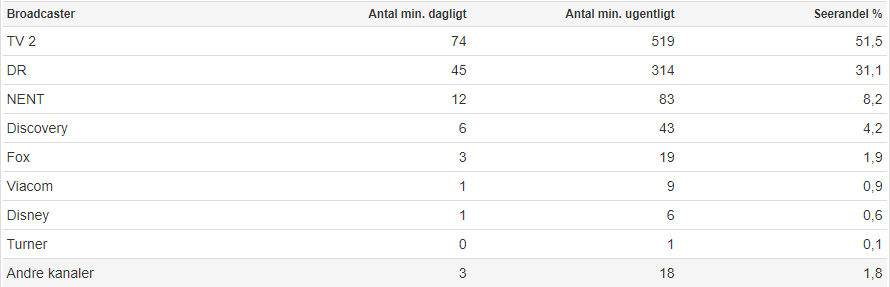
\includegraphics[scale = 0.75]{images/Seertal.png}
    \caption{Seertid i uge 3 2020}
    \label{fig:Seertid}
\end{figure}
Det første tal der ses i figur \ref{fig:Seertid} viser, hvor mange minutter den gennemsnitlige dansker bruger på en given broadcasters tv-kanaler. Det næste tal viser hvor mange minutter det er om ugen, og det sidste tal viser, hvor stor en seerandel den givne broadcaster besidder på markedet for perioden. 
%Problemet
Som det ses har TV2 en stor seerandel, og af den grund består en vigtig del af deres indkomst af de reklamer de sender mellem deres programmer.  Men den indkomst kan blive bedre endnu, hvis de bliver bedre til at optimere tiden mellem deres programmer, vurderer TV2. Og det er netop dette problem som danner grundlag for vores case.

\subsection{Redegørelse for den udleverede case}
Når et program slutter på en af TV2s kanaler, bliver der vist rulletekster for at kreditere de medvirkende i programmet. Disse rulletekster tager dog i nogle tilfælde op til 30 sekunder, hvilket er 30 sekunder for meget. TV2 har vurderet, at hvis man kan frigøre disse 30 sekunder fra rulletekster, og bruge dem på reklamer i stedet, vil de kunne tjene op imod 60 millioner DKK om året. \cite{url_case}

Netop dette vil TV2 gøre ved at digitalisere krediteringerne, så de kan ses på nettet eller en app. For Udover at kunne sende flere reklamer mellem deres programmer, vil TV2 også have muligheden for at kreditere alle, og ikke bare de vigtigste efter endt program. I de fleste tilfælde var 30 sekunders rulletekster nemlig ikke nok til at kreditere alle medvirkende, så derfor har TV2 været nødt til at prioritere, hvilket selvfølgelig fører til at nogle krediteringer bliver glemt. Digitaliseres krediteringerne, vil alle kunne blive krediteret ligeligt, og der vil derved ikke være nogen som bliver glemt, fordi deres rolle er mindre vigtig.

Vores opgave i denne case er at skabe netop denne digitalisering af krediteringer. Det er vores opgave at udvikle et software system som kan tilføje, fjerne og redigere krediteringer i en database, hvortil vi har formuleret en problemformulering, som skal hjælpe os med at få udarbejdet en løsning på TV2s problematik med kreditering.

\subsection{Formålet med opgaven}
Formålet med det system vi har udviklet, er at gøre det lettere for producere, administratorer og TV2 som virksomhed, at kunne redigere og holde styr på krediteringer. Derudover er formålet med projektopgaven også at vi som gruppe skal forbedre vores evner inden for programmering af softwaresystemer og håndtering af databaser. Samtidigt med at vi videre udvikler vores kompetencer inden for gruppearbejde, og opsætning af et struktureret arbejdsmiljø.

Vores semesterprojekt er inddelt i to iterationer, 
\subsection{Problemanalyse}
\subsection{Problemformulering}
\subsection{Afgrænsninger}